\documentclass[a4paper,final]{memoir}

%\setlength{\parindent}{0pt}
% Language and encoding
\usepackage[utf8]{inputenc}
\usepackage[T1]{fontenc}
\usepackage[english]{babel}
\usepackage[protrusion=true,expansion=true]{microtype} % better typography

% Math
\usepackage{amsmath,amssymb,amsfonts,amsthm,latexsym}


\newtheorem{thm}{Theorem}[chapter]
\theoremstyle{definition}

%\newtheoremstyle{mydefstyle}
%  {3\topsep} % Space above
%  {3\topsep} % Space below
%  {} % Body font
%  {} % Indent amount
%  {\bfseries} % Theorem head font
%  {} % Punctuation after theorem head
%  {.5em} % Space after theorem head
%  {} % Theorem head spec (can be left empty, meaning `normal')
%
%\theoremstyle{mydefstyle}
\newtheorem{defn}{Definition}[chapter]
%\newtheorem{examp}[thm]{Example}

\newcommand{\bbN}{\mathbb N} %the natural numbers
\newcommand{\bbZ}{\mathbb Z} %the integers
\newcommand{\bbQ}{\mathbb Q} %the rational numbers
\newcommand{\bbR}{\mathbb R} %the real numbers
\newcommand{\bbC}{\mathbb C} %the complex numbers

%\providecommand*{\listingautorefname}{Listing}

% Graphic stuff
\usepackage[pdftex]{graphicx}
\usepackage[usenames,dvipsnames,table]{xcolor}
\definecolor{shade}{RGB}{245,245,245}
\usepackage[pdftex,colorlinks=true]{hyperref}
\hypersetup
{
    bookmarksnumbered,
    linkcolor=RoyalBlue,
    anchorcolor=RoyalBlue,
    citecolor=RoyalBlue,
    urlcolor=RoyalBlue,
    pdfstartview={FitV},
    pdfdisplaydoctitle
}
\usepackage{pgfplots}

% Tables
\usepackage{booktabs}
\usepackage[hang,small,bf]{caption}

% Debug, etc.
\usepackage{todonotes}

% Numbering
\setsecnumdepth{subsection}
\maxtocdepth{subsection}
\numberwithin{equation}{chapter}
\numberwithin{figure}{chapter}
\numberwithin{table}{chapter}

% Computer science stuff
\usepackage{clrscode3e}
\usepackage{verbatim}
\newcommand{\mono}[1]{{\ttfamily#1}}
\usepackage{listings}
\lstset
{
    tabsize=2,
    numbers=left,
    breaklines=true,
    backgroundcolor=\color{shade},
    framexleftmargin=0.05in,
    basicstyle=\ttfamily\small,
    numberstyle=\tiny,
    keywordstyle=\color{RoyalBlue},
    stringstyle=\color{Maroon},
    commentstyle=\color{ForestGreen}
}


% Document meta stuff
\newcommand{\horrule}[1]{\rule{\linewidth}{#1}}
\makeevenfoot{plain}{}{}{\thepage}
\makeoddfoot{plain}{}{}{\thepage}

\begin{document}

\frontmatter

\begin{titlingpage}
\begin{center}

\usefont{OT1}{bch}{b}{n}
\normalfont \normalsize
\textsc{Department of Computer Science, University of Copenhagen} \\ [25pt]
\horrule{0.5pt} \\ [0.4cm]
\huge Introduction to Compact Name-Independent Routing with Minimum Stretch\\
\horrule{2pt} \\ [0.5cm]
\normalfont \normalsize
Henrik Bendt \& Jonas Brunsgaard \\ \normalsize
\today

\end{center}
\end{titlingpage}

%\thispagestyle{empty}

\tableofcontents

\pagestyle{Ruled}
\chapterstyle{hangnum}
\mainmatter

\newpage
%\chapter{Introduction}
\label{sec:introduction}

Finding the shortest path between a vertex pair in a graph is one
of the most fundamental computational graph problems. Papers like
Dijkstra\cite{Dijkstra59anote} and Bellman-Ford\cite{bellman} presents
algorithms able to determine the shortest path for a single vertex pair, but
these algorithms does not scale well, as they need to visit every vertex in
the graph to come up with a result. Thus, these algorithms are a poor choice
for applications that needs to answer shortest path queries for large graphs
extremely fast.

Now suppose you are given a connected weighted undirected graph $G=(V,E)$
consisting of $n$ vertices and $m$ edges, and you are asked to come up with a
solution able to answer shortest path queries extremely fast.

The naive solution is to compute the shortest path between every vertex pair
$(u,v) \in V \times V$ and store the information in a lookup table using
$(u,v)$ as key for the entry. Subsequent distance queries can be answered in
constant time simply by performing a lookup in the hash table.
However, there are strong objections to this naive solution.

First of all the preprocessing time may simply be too long, and secondly,
even if one is willing to wait for the preprocessing to finish, the size of
the final lookup table may be too large to store efficiently. Using Thorups
shortest path algorithm for undirected graphs\cite{thorupsssp}, which offers
$O(m)$ time complexity, to compute the distances from each vertex $v\in V$,
one gets a time complexity of $O(nm)$ while $O(n^2)$ space is required by the
lookup table.

If one can settle for approximated distances instead of exact ones,
approximate distance oracles is the better alternative for undirected
graphs. Approximate distance oracles is a data structure presented by Thorup
and Zwick\cite{tu}, it offers much better space and construction time
complexities, while still being able to answer shortest path queries in
constant time.

More precisely the paper describe for any integer $k \leq 1$, a preprocessing
algorithm that runs $O(kmn^{1/k})$, producing a data structure of size
$O(kn^{1+1/k})$. The data structure can return approximate distances of a
finite stretch $t$. An estimated distance $\hat{\delta}(u,v)$ from $u$ to $v$
is said to be within the stretch $t$ if and only if $\delta(u,v)\leq
\hat{\delta}(u,v)\leq t \cdot\delta(u,v)$ where $\delta(u,v)$ denotes the
exact shortest distance. The actual stretch of the produced estimates is
at most $2k-1$, but it may be as low as $1$. Thorup and Zwick does not discuss
this further.

In this report I study - through experiments - the average actual stretch of
distances produced by \emph{Stretch-3} ($k=2$) approximate distance oracles. A
high quality implementation of the algorithm has been developed to conduct
the experiments, and has been used to compute approximate distance oracle
data structures for graphs representing internet topologies and road networks.

Using a sample of vertex pairs from each graph, and comparing the actual
shortest path against the approximated shortest path in the sample, I show the
average actual stretch for these internet topologies and road networks. The
goal is to provide data that indicates what actual stretch to expect, if you
apply approximate distance oracles to these classes of graphs.

The rest of the article is organized as follows: In the next short chapter I
introduce some basic background material. Then, \autoref{sec:ado} presents an
introduction to approximate distance oracles. In \autoref{sec:implementation}
I discuss obstacles and solution regarding the implementation and development
process. Finally in \autoref{sec:experiments} I conduct and discuss my
experiments before I present my conclusions in \autoref{sec:conclusion}.




\section{Lets talk a bit about routing}

\begin{frame}[fragile]
  \frametitle{Routing Scheme}
    A routing scheme is a distributed algorithm that allows any
    source node to route messages to any destination node, given
    destination node's name

    \begin{description}
        \item[Input] a network $G$ (a weighted connected graph)
        \item[Output] a routing scheme for G
    \end{description}
\end{frame}

\begin{frame}{XY-routing}
  \begin{figure}
    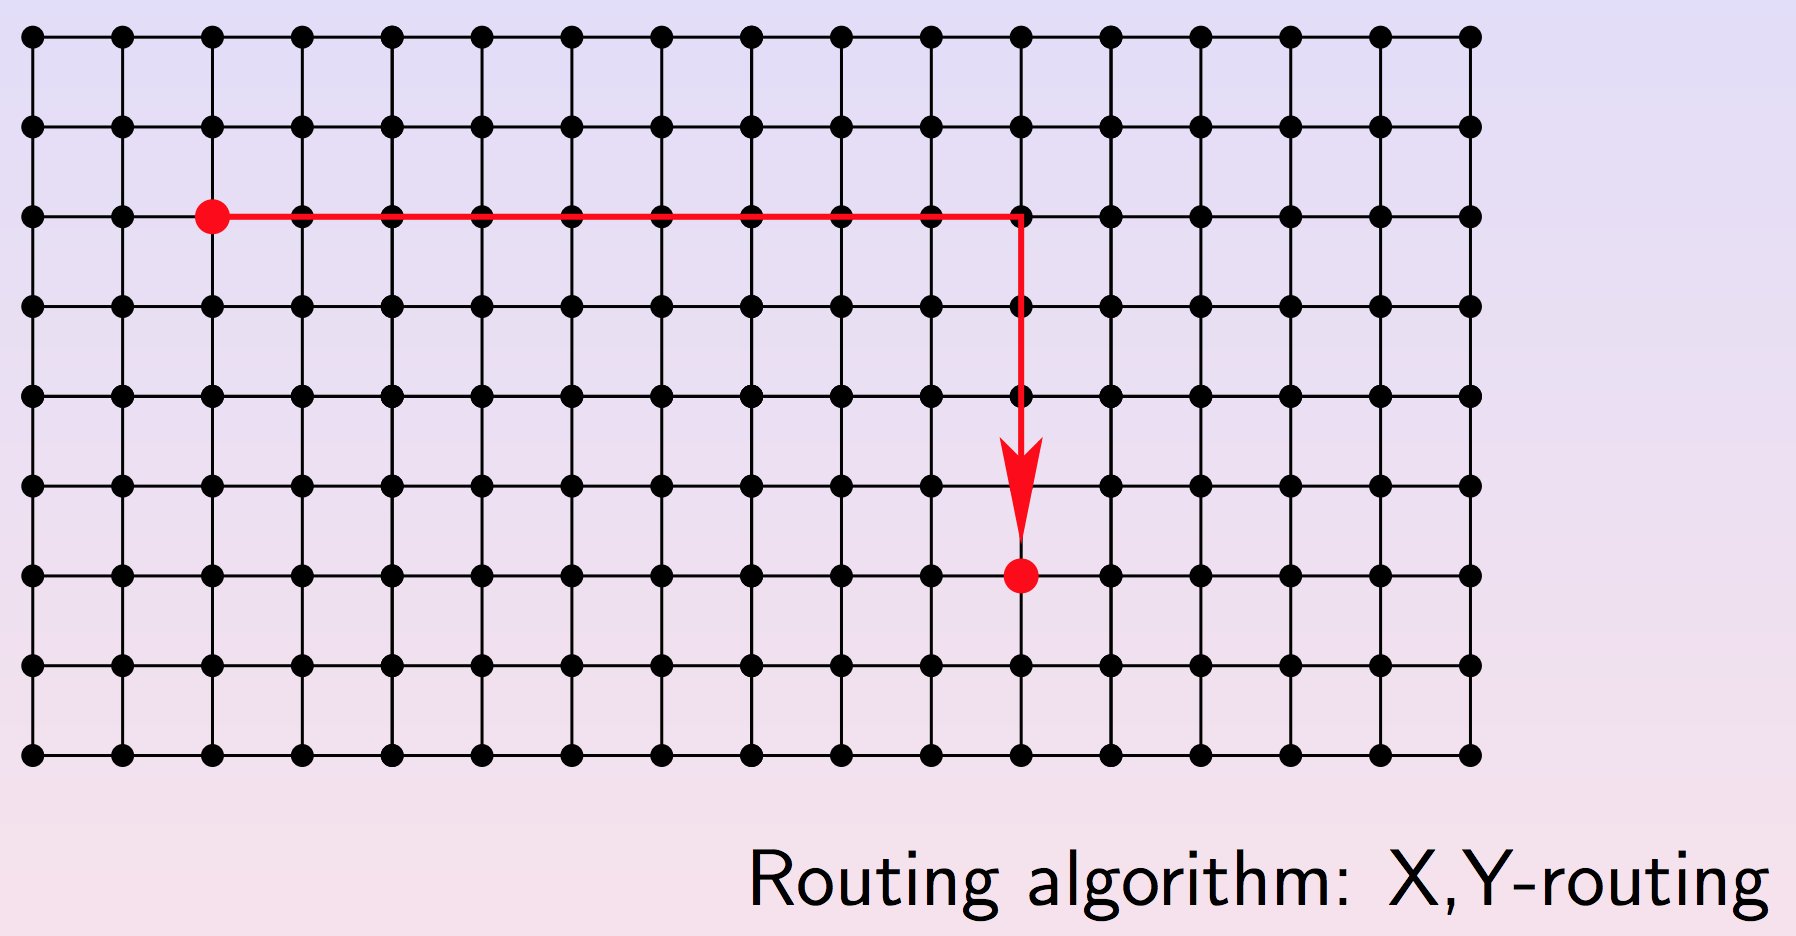
\includegraphics[scale=0.3]{images/xyrouting.png} 
  \end{figure}
\end{frame}

\begin{frame}[fragile]
  \frametitle{Routing Scheme}
     
  \begin{block}{Example: Trivial routing on min cost paths}
      \begin{itemize}
        \item On each node, for each of the possible $(n-1)$ destinations,
        store a port number leading to the next node on a min cost path to the
        destination.
        \item Requires each node to store $\Omega (n\; log\; n)$ bits.
        \item Does not scale very well.
      \end{itemize}
  \end{block}
\end{frame}

\begin{frame}[fragile]
  \frametitle{Minimizing parameters}
  When working with routing, two factors are normally of interest:
  \begin{description}
    \item[Stretch] The max ratio over all source-destination pairs between the
        cost of the path taken by the routing scheme and the cost of a min
        cost path.
    \item[Memory] The max number of bits over all nodes stored for the routing
        scheme. (ballanced is preferred)
  \end{description}
\end{frame}

\begin{frame}[fragile]
  \frametitle{Labeled Routing or Name-Independent Routing}

  In labeled routing we can choose a label for each vertex.
  Lets use coordinates. Now we can easily route. If an aversery
  label the vertices randomly, routing gets harder.

  \begin{figure}
    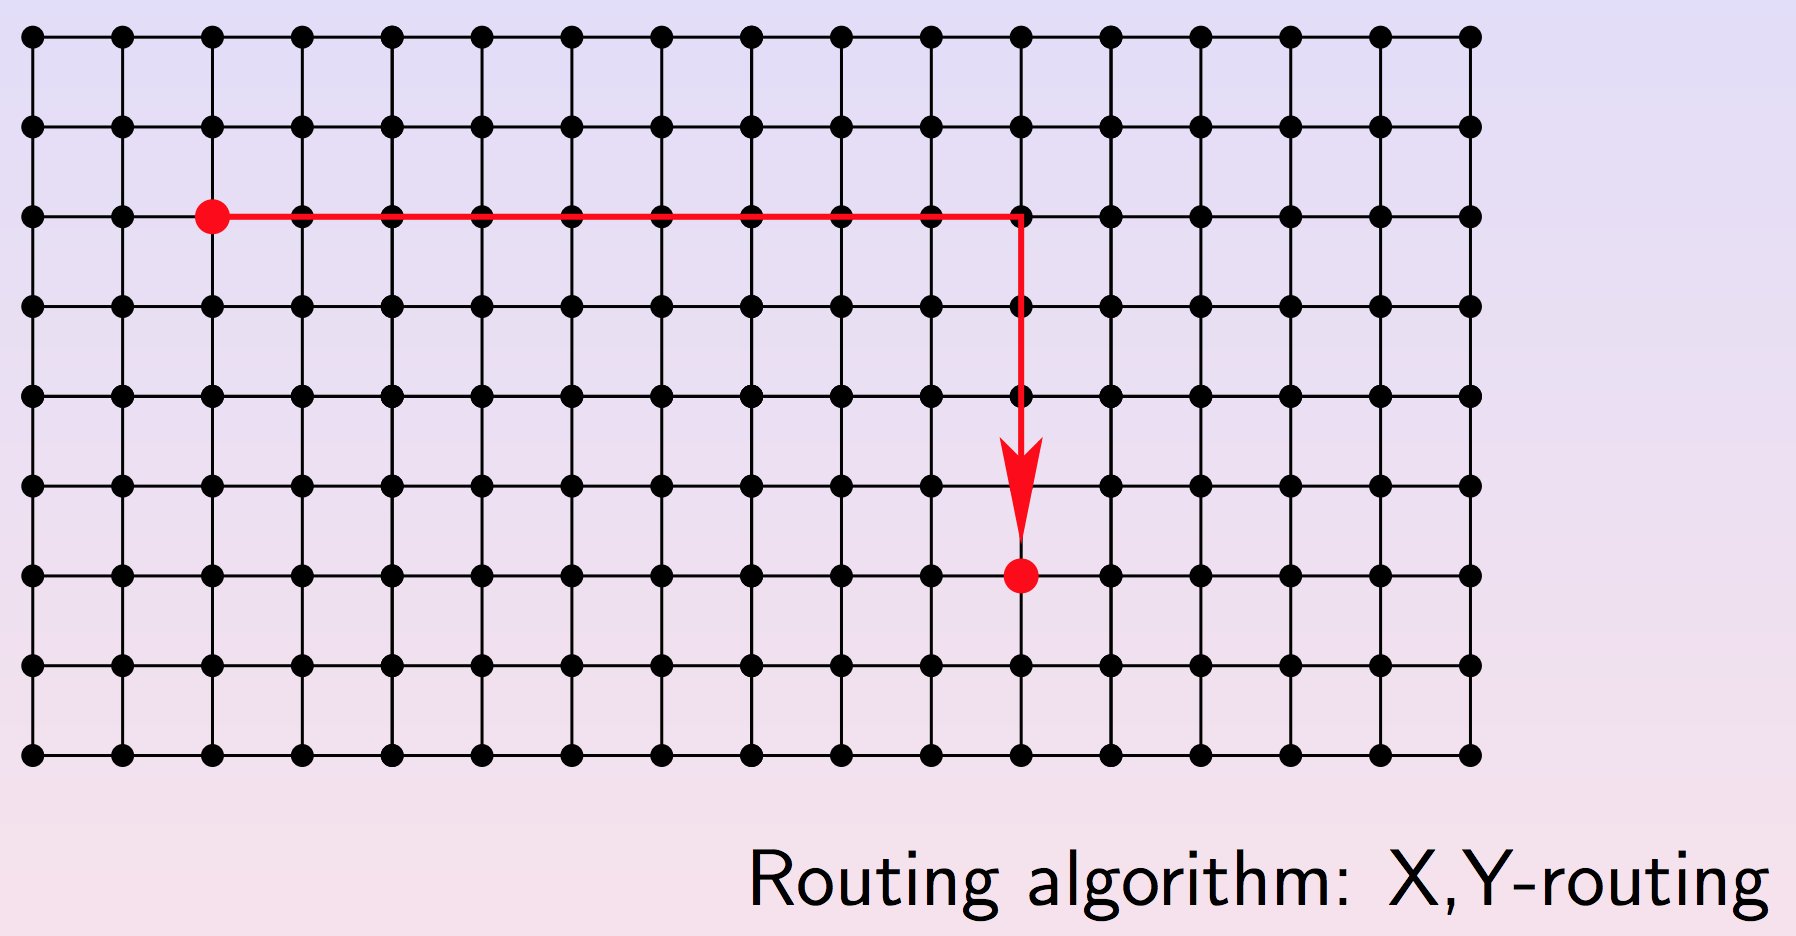
\includegraphics[scale=0.3]{images/xyrouting.png} 
  \end{figure}
\end{frame}




\begin{frame}[fragile]
  \frametitle{Name-Independent Rounting with min stretch}
    Given a weighted undirected network with arbitrary node names, we present
    a compact routing scheme, using a $\tilde{O}(\sqrt{n})$ space routing
    table at each node and routing along paths of stretch 3.

    It is known that no compact routing using $o(n)$ space per node can route
    with stretch below 3. Also, it is known that any stretch below 5 requires
    $\Omega(\sqrt{n})$ space per node.
\end{frame}

\begin{frame}[fragile]
  \frametitle{Setup}
    Consider an $n$-node weighted undirected graph $G=(V,E,\omega)$.

    Each node $v\in V$:
    \begin{itemize}
        \item is given a unique name with $O(log\; n)$ bits.
        \item each outgoing edge is given a unique port name in $\{1,\dots,deg(v)\}$.
    \end{itemize}
\end{frame}

\newpage
\section{The Stretch 3 Scheme}
We shall firstly introduce a stretch 3 scheme for complete graphs and then generalize this to generic graphs.

\subsection{Vicinity Balls}
We introduce vicinity balls as the notion of areas containing the $k$ closest nodes. For every integer $k \geq 1$, and for a node $u \in V$, let the \textit{vicinity} of $u$, denoted by $B_k(u)$, be the set consisting of $u$ and the $k$ closest nodes to $u$.

Set $k=[4 \sqrt{n}log\; n]$ and denote $B(u) = B_k(u)$. Denote $b(u)$ the radius of $B(u)$, $b(u)=max_{w\in B(u)} d(u,w)$.

\subsection{Coloring}
We introduce coloring.
Partition nodes into the color sets $C_1,\dots,C_{\sqrt{n}}$, with the following properties:
\begin{enumerate}
    \item Every color-set has at most $2 \sqrt{n}$ nodes.
    \item Every node has in its vicinity at least one node from every color-set.
\end{enumerate}

If node $u\in C_i$, it has ``color $i$'' and we denote this $c(u)=i$. The coloring can be done in polynomial time.

If every node independently chooses a random color, the properties holds with high probability.
%TODO prove this

\subsection{Hashing Names To Colors}
Assuming a mapping $h$ from node names to colors is balanced such that at most $O(\sqrt{n})$ names map to the same color. Each node $u\in V$ should be able to compute $h(w)$ for any destination $w$ in constant time. Note that this hashing is for node names and not the node itself. Thus a node now has a node color and a name color.

\section{Stretch 3 for Complete Graph}
\subsection{Storing}
Every node $u$ stores the following:
\begin{enumerate}
    \item The names of all the nodes in the vicinity $B(u)$ and what port number to use to reach them.
    \item The names of all nodes $v$ such that $c(u)=h(v)$ and what port number to use to reach them.
\end{enumerate}

\subsection{Routing}
Routing from $u$ to $v$ is done in the following manner:
\begin{enumerate}
    \item If $v\in B(u)$ or $c(u)=h(v)$, then $u$ routes directly to $v$ with stretch 1 (i.e. min cost)
    \item Otherwise, $u$ forwards the packet to $w\in B(u)$ such that $c(w)=h(v)$. Then from $w$ the packet goes directly to $v$.\\
        The stretch is at most $3$ since $d(u,w) + d(w,v) \leq d(u,v)+2d(u,v)$.
\end{enumerate}

%TODO include example

\chapter{Stretch 3 Scheme (for all graphs)}
We now generalizes the stretch 3 scheme for complete graphs to generic graphs. To do this, we introduce routing on trees, landmarks and partial shortest path trees.

\subsection{Routing on Trees}
From Fraigniaud and Gavoille 2001 \cite{fraigniaudGavoille2001}, Thorup og Zwick 2001B \cite{thorupZwick2001b}, we have:

For every weighted tree $T$ with $n$ nodes there exists a labeled routing scheme that, given any destination label, routes optimally on $T$ from any source to the destination. The storage per node in $T$, the label size, and the header size are $O(log2 n/ log log n)$ bits. Given the information of a node and the label of the destination, routing decisions take constant time, by Lemma 3.3 \cite{compactNameIndepRouting}[37:6].

For a tree $T$ containing a node $v$, let $\mu(T, v)$ denote the routing information
stored at node $v$ and $\lambda(T, v)$ denote the destination label of $v$ in $T$ as defined by the
labeled routing scheme of Lemma 3.3 \cite{compactNameIndepRouting}[37:6].

\subsection{Landmarks}
Designate one color to be the landmark color. Let $L$ denote the set of nodes with this color. Because of the way coloring works we have that $|L| \leq 2 \sqrt{n}$ and that for every $v\in V$, $B(v)\cap L \neq \emptyset$.

For a node $v\in V$, let $\ell_v$ denote the closest landmark node in $B(v)$.

\subsection{Partial shortest path trees}
For any node $u$, let $T(u)$ denote a singlesource minimum-cost-path tree rooted at $u$. In a partial shortest path tree, every node $v$ maintains $\mu(T(u),v)$ if and only if $u \in B(v)$. Notice that the set of nodes that maintain $\mu(T(u),\dot)$ is a subtree of $T(u)$ that contains $u$.\\

%\begin{quote}[\texttt{Lemma 3.4}]
%    \textit{If $x \in B(y)$, then given the label $\lambda(T(x), y)$, node $x$ can
%    route to node $y$ along a minimum cost path.}
%\end{quote}
%TODO: Prove this

\texttt{Lemma 3.4}. \textit{If $x\in B(y)$, then given the label $\lambda(T(x),y)$, node $x$ can route to node $y$ along a min cost path.}

\texttt{Proof}. By Property 3.1 for any node $w$ on the min cost path of $T(x)$ between $x$ and $y$ we have $x\in B(w)$. Thus every node $w$ on this path maintains $\mu(T(x),w)$

\subsection{Storing}\label{subsec:storing}
Every node $u$ stores the following
\begin{enumerate}
    \item For every $w\in B(u)$, the name $w$ and the port name $u\rightarrow y$, where $(u\rightarrow y)$ is the port number to use to get to node $y$, which is the next hop on a min cost path from $u$ to $w$.
    \item For every landmark node $\ell \in L$, routing information $\mu(T(\ell),u)$ and label $\lambda(T(\ell),\ell)$ of the tree $T(\ell)$.
    \item For every node $x\in B(u)$, routing information $\mu(T(x),u)$ of the tree $T(x)$.
    \item For every node v such that $c(u) = h(v)$, store one of the following two options that produces the minimum cost path out of the two:
    \begin{enumerate}
        \item[a] Store the labels $<\lambda(T (\ell_v), \ell_v ), \lambda(T (\ell_v), v)>$. The routing path in this case would be from $u$ to $\ell_v \in B(v)$ using $\lambda(T (\ell_v), \ell_v)$ on the tree $T (\ell_v)$, and from $\ell_v$ to $v$ using $\lambda(T (\ell_v), v)$ on the same tree $T (\ell_v)$.

        \item[b] Let $P(u, w, v)$ be a path from u to v composed of a minimum cost path from $u$ to $w$, and of a minimum cost path from $w$ to $v$ with the followingproperties: $u \in B(w)$, and there exists an edge $(x, y)$ along the minimum cost path from $w$ to $v$ such that $x \in B(w)$ and $y \in B(v)$. If such paths exists, choose the lowest cost path $P(u, w, v)$ among all these paths and store the labels $<\lambda(T (u), w), x, (x \rightarrow y), \lambda(T (y), v)>$.\\
        The routing path in this case would be from $u$ to $w$ on $T(u)$ using $\lambda(T (u), w)$. This part is possible by Lemma 3.4 on $u \in B(w)$. Then from $w$ to $y$ since $x \in B(w)$ and the port number $(x \rightarrow y)$ is stored. Finally from $y$ to $v$ on $T(y)$ using $\lambda(T (y), v)$. This part is possible by Lemma 3.4 on $y \in B(v)$.
    \end{enumerate}
\end{enumerate}

\subsection{Routing}
Routing from u to v is done in the following manner:
\begin{enumerate}
    \item If $v \in B(u)$ or $v \in L$ ($v$ is a landmark node) or $c(u) =
        h(v)$, then $u$ routes to $v$ using its own information.
    \item Otherwise, $u$ forwards the packet to $w \in B(u)$ such that
        $c(w) = h(v)$. Then from $w$ the packet goes to $v$ using $w$’s
        routing information.
\end{enumerate}

\section{Theorem 3.5}
\textit{Let $s,t\in V$ be any two nodes. The route of the scheme from $s$ to $t$ has stretch at most 3.}

\texttt{Proof}. There are three cases to consider:
\subsection{Analysis}
\begin{enumerate}
    \item \textit{The taget is inside the source vicinity}: If $t\in B(s)$ or $t\in L$, then $s$ routes on a minimum cost path directly to $t$.

    Otherwise, let $z$ be a node such that $z\in B(s)$ and $c(z)=h(t)$. For the case $c(s)=h(t)$, set $z=s$. Let $p(z,t)$ be the cost of the path chosen by $z$ as the lowest cost   path from $z$ to $t$ (from options 4(a) and 4(b)). Then:
    \item \textit{The source and target vicinities are far apart}: On every min cost path from $s$ to $t$ there is a node $y$ such that $y\not\in B(s)$ and $y\not\in B(t)$. In this case, $b(s)+b(t)\leq d(s,t)$.

    From 4(a) the cost $d(s,z)+p(z, t)$ of the path taken by the routing scheme is bounded by the cost of the path $s\leadsto z\leadsto \ell_t\leadsto t$, where $u\leadsto v$ is the min cost path from $u$ to $v$.\\
    Thus $d(s,z)+p(z,t) \leq d(s,z)+d(z,\ell_t)+d(\ell_t,t) \leq b(s) + [b(s) + d(s,t) + b(t)] + b(t) \leq 3d(s,t)$.
    \item \textit{The source and atarget vicinities are close}: There exists a min cost path in which every node is in $B(s)\cup B(t)$. Let $(x,y)$ be an edge on this path such that $x\in B(s)$ and $y\in B(t)$. From 4(b), the cost $d(s,z)+p(z,t)$ of the path taken is bounded by the cost of path $s\leadsto z\leadsto x\rightarrow y \leadsto t$.\\
    Thus $d(s,z)+p(z,t) \leq d(s,z) + d(z,s) + d(s,t) \leq b(s)+b(s)+d(s,t)\leq 3d(s,t)$.
\end{enumerate}
The three cases is depicted in \autoref{fig:threecases}.

\begin{figure}[htbp]
    \centering
    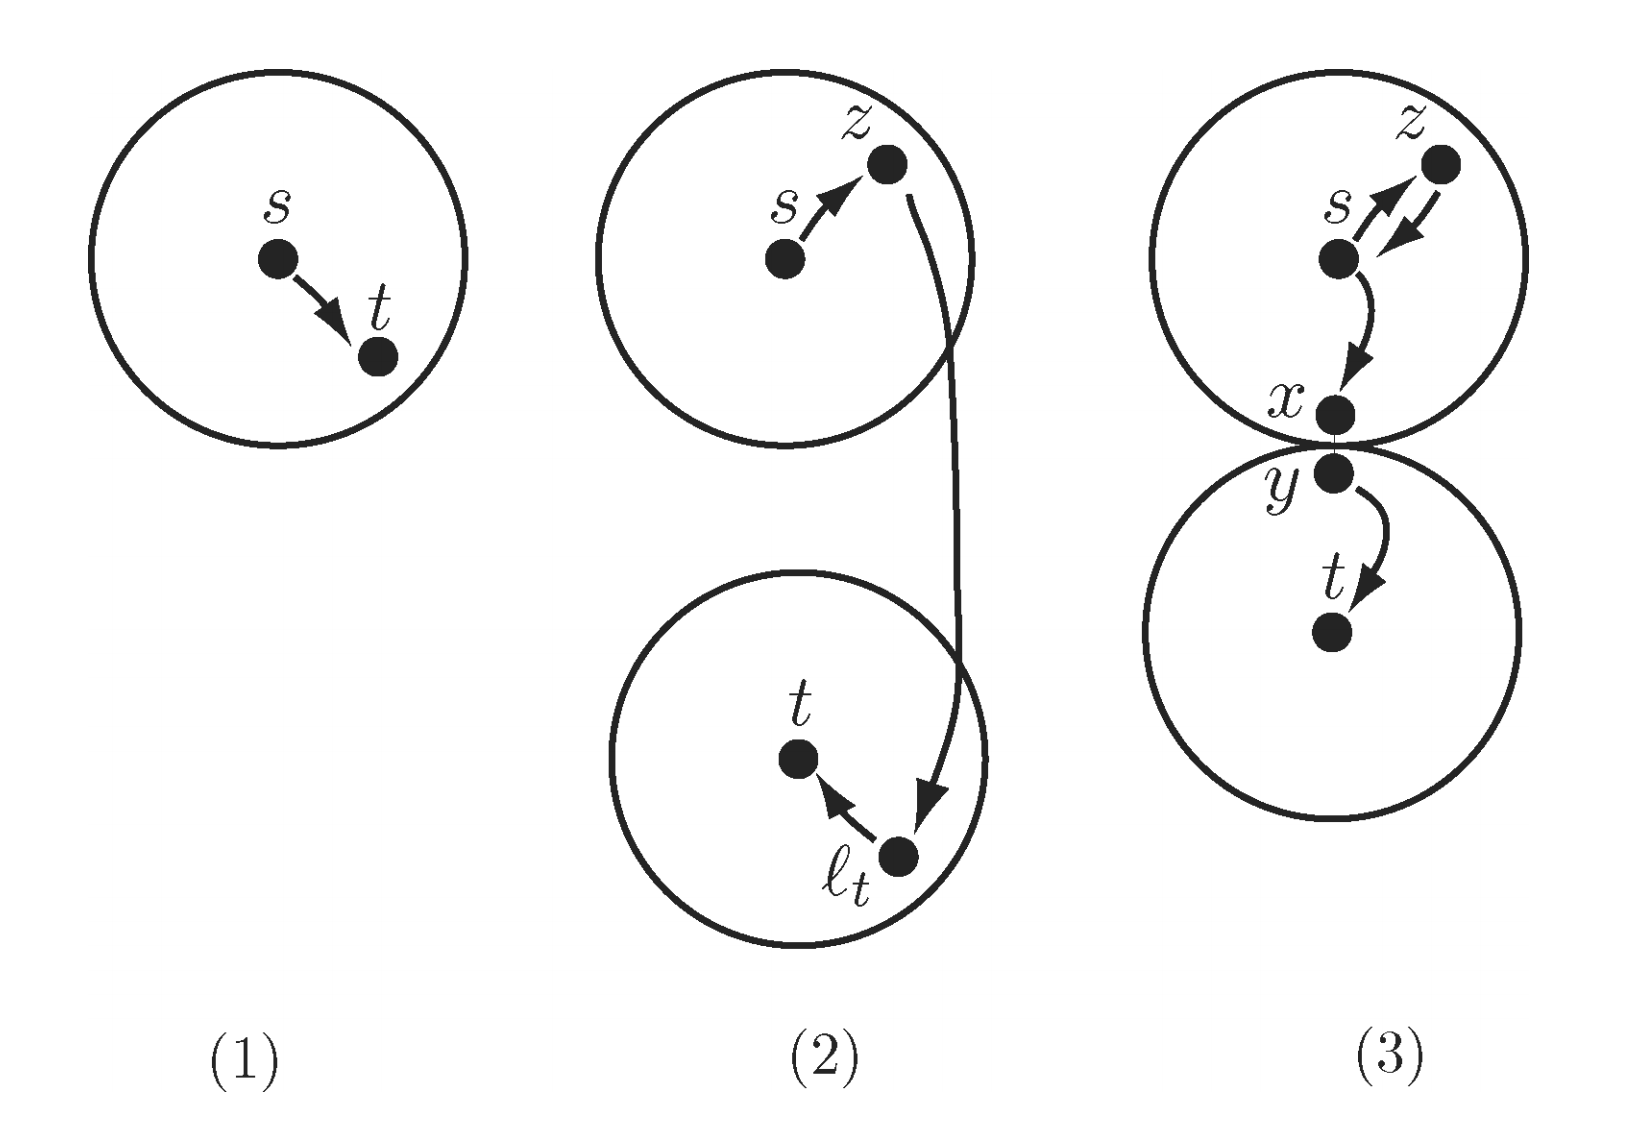
\includegraphics[scale=0.3]{images/threecases.png} 
    \caption{An illustration of the three cases described in the analysis.}
    \label{fig:threecases}
\end{figure}


\section{Results}
The routing information stored at each node in \ref{subsec:storing} is bounded by
\begin{enumerate}
    \item $\tilde{O}(\sqrt{n})$ as $|B(u)| = \tilde{O}(\sqrt{n})$.
    \item $\tilde{O}(\sqrt{n})$ as each node will participate in $\tilde{O}(\sqrt{n})$ trees and thus its total tree routing information is of size $\tilde{O}(\sqrt{n})$ by Lemma 3.3.
    \item $\tilde{O}(\sqrt{n})$ by the same logic as for the above.
    \item $\tilde{O}(\sqrt{n})$ as for a node $u$ the number of nodes $v$ such that $c(u) = h(v)$ is bound by $\tilde{O}(\sqrt{n})$ (by the property 3.2 and the assumption of the hashing being balanced), and the lables stored are of $\tilde{O}(1)$ size.
\end{enumerate}
giving the a total bound on size of $\tilde{O}(\sqrt{n})$.

The described stretch 3 scheme has the following bounds:
\begin{description}
    \item[Stretch] 3
    \item[Header size] $O(log^2/log\;log\;n)$ bits
    \item[Routing information stored per node] $\tilde{O}(\sqrt{n})$ bits
    \item[Routing] $O(1)$ time
    \item[Construction time] $\tilde{O}(n|E|)$
\end{description}
where the routing information stored per node 

Improves the stretch of Arias et al. [2003]\cite{ariasEtAl2003} from 5 to 3, the known lower bound and answers the open problem from 1989 [Awerbuch et al. 1990]. %TODO cite

\bibliographystyle{amsplain}
\bibliography{references}


\end{document}
